% !TeX root = Protokoll.tex

\section{Hysterese des Magneten}
Vor der Aufnahme der roten und blauen Spekrallinie der Cd-Spekrallampe,
muss zunächst die Hysterese des verwendeten Elektromagneten aufgenommen
werden. Die aufgenommenen Messwerte für die, mittels Hall-Sonde gemessene,
magnetische Flussdichte sind in Abhängigkeit der eingestellten Stromstärke
in den Tabellen \ref{tab:hysterese_zunehmend} und \ref{tab:hysterese_abnehmend}
aufgeführt. Dabei wurde die Stromstärke während der erste Messung sukzessive
erhöht und während der zweiten verringert.
Desweiteren wurden die Messwerte in \cref{fig:hysterese_messung_i_zunehmend}
respektive \cref{fig:hysterese_messung_i_abnehmend} grafisch dargestellt.
Für den Vergleich der beiden Messungen wurden jeweils beide Messreihen
dargestellt, jedoch wurden die zusätzlich dargestellten Regressionsgraden
nur auf Grundlage jeweils einer Messung bestimmt.

\begin{table}[!h]
	\centering
	\begin{tabular}{cccc}
		\toprule
		Stromstärke & magn. Flussdichte & Stromstärke & magn. Flussdichte\\
		$I$/\si{\ampere} & $B$/\si{\milli\tesla} & $I$/\si{\ampere} & $B$/\si{\milli\tesla}\\
\midrule
		\num{0.0(5)} & \num{6(1)} & \num{9.0(5)} & \num{553(1)}\\
		\num{1.0(5)} & \num{72(1)} & \num{10.0(5)} & \num{614(1)}\\
		\num{2.0(5)} & \num{136(1)} & \num{11.0(5)} & \num{674(1)}\\
		\num{3.0(5)} & \num{189(1)} & \num{12.0(5)} & \num{733(1)}\\
		\num{4.0(5)} & \num{248(1)} & \num{13.0(5)} & \num{787(1)}\\
		\num{5.0(5)} & \num{305(1)} & \num{14.0(5)} & \num{813(1)}\\
		\num{6.0(5)} & \num{371(1)} & \num{15.0(5)} & \num{863(1)}\\
		\num{7.0(5)} & \num{431(1)} & \num{16.0(5)} & \num{903(1)}\\
		\num{8.0(5)} & \num{491(1)} & \num{17.0(5)} & \num{928(1)}\\
		\bottomrule
	\end{tabular}
	\caption{Messwerte der magnetischen Flussdichte, die in Abhängigkeit der angelegten Stromstärke
                        aufgenommen wurden, um die Hysterese des verwendeten Magneten zu bestimmen. 
                        In dieser Messung wurde die Stromstärke sukzessive erhöht. \label{tab:hysterese_zunehmend}}
\end{table}

\FloatBarrier
\begin{figure}[!h]
\centering
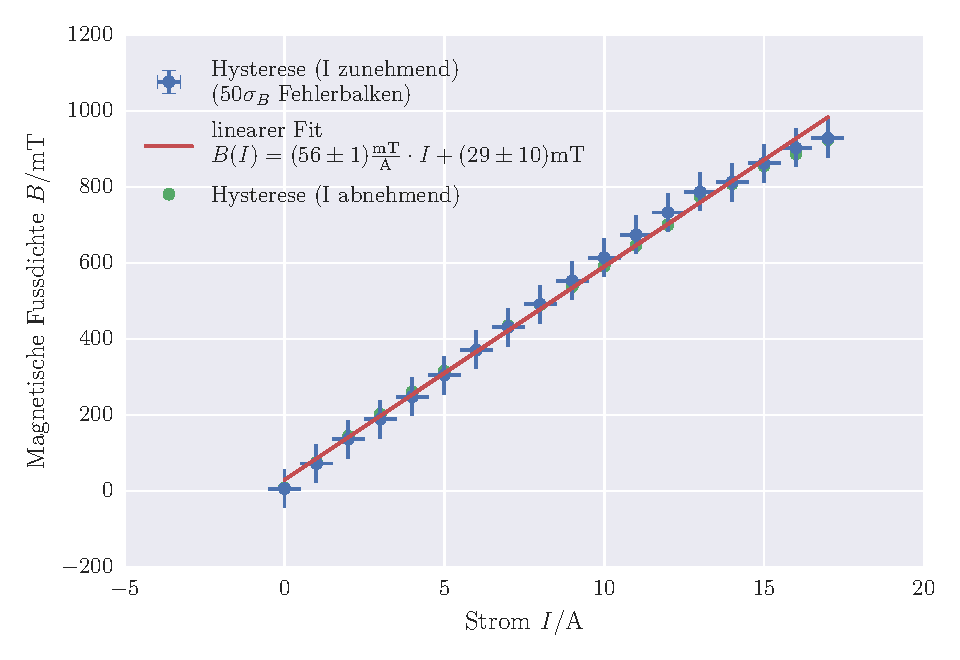
\includegraphics[scale=1]{../Grafiken/Hysterese_Messung_I_zunehmend.pdf}
\caption{Grafische Darstellung der in Abhängigkeit von der Stromstärke $I$
         aufgenommenen Messwerte der magnetischen Flussdichte $B$.
         Die zusätzlich dargestellte Regressionsgerade wurde aus den mit
         Fehlerbalken dargestellten Messwerten (für zunehmenden Strom) bestimmt.
         Die übrigen Messwerte (für abnehmenden Strom) sind für den Vergleich
         der beiden Messreihen dargestellt.
         \label{fig:hysterese_messung_i_zunehmend}}
\end{figure}
\FloatBarrier

\begin{table}[!h]
	\centering
	\begin{tabular}{cccc}
		\toprule
		Stromstärke & magn. Flussdichte & Stromstärke & magn. Flussdichte\\
		$I$/\si{\ampere} & $B$/\si{\milli\tesla} & $I$/\si{\ampere} & $B$/\si{\milli\tesla}\\
\midrule
		\num{0.0(5)} & \num{8(1)} & \num{9.0(5)} & \num{538(1)}\\
		\num{1.0(5)} & \num{75(1)} & \num{10.0(5)} & \num{591(1)}\\
		\num{2.0(5)} & \num{144(1)} & \num{11.0(5)} & \num{646(1)}\\
		\num{3.0(5)} & \num{202(1)} & \num{12.0(5)} & \num{701(1)}\\
		\num{4.0(5)} & \num{261(1)} & \num{13.0(5)} & \num{775(1)}\\
		\num{5.0(5)} & \num{315(1)} & \num{14.0(5)} & \num{808(1)}\\
		\num{6.0(5)} & \num{371(1)} & \num{15.0(5)} & \num{856(1)}\\
		\num{7.0(5)} & \num{435(1)} & \num{16.0(5)} & \num{887(1)}\\
		\num{8.0(5)} & \num{490(1)} & \num{17.0(5)} & \num{925(1)}\\
		\bottomrule
	\end{tabular}
	\caption{Messwerte der magnetischen Flussdichte, die in Abhängigkeit der angelegten Stromstärke
                        aufgenommen wurden, um die Hysterese des verwendeten Magneten zu bestimmen. 
                        In dieser Messung wurde die Stromstärke sukzessive verringert. \label{tab:hysterese_zunehmend}}
\end{table}

\FloatBarrier
\begin{figure}[!h]
\centering
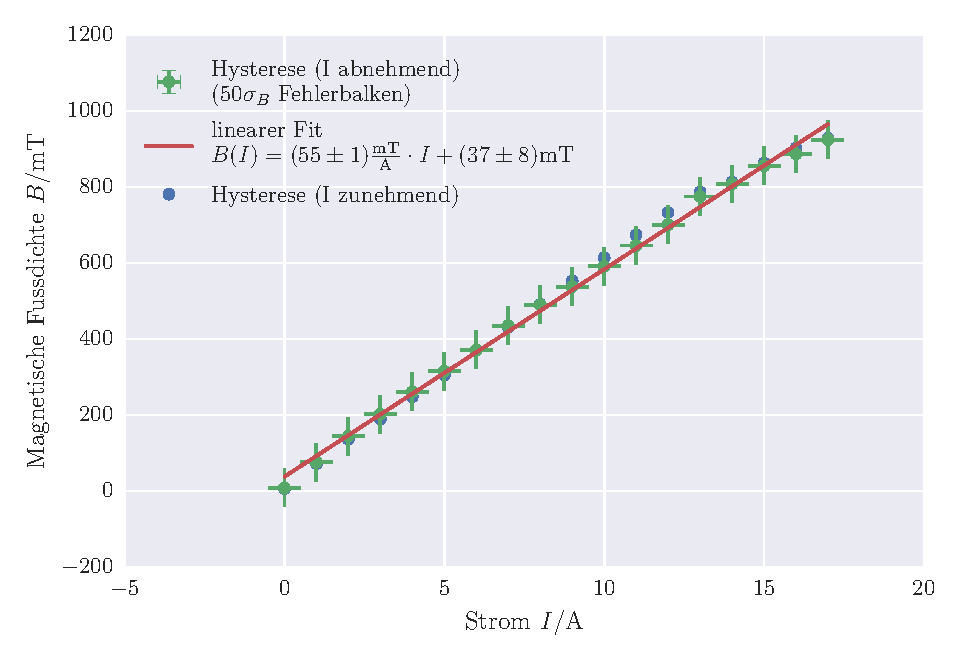
\includegraphics[scale=1]{../Grafiken/Hysterese_Messung_I_abnehmend.pdf}
\caption{\label{fig:hysterese_messung_i_abnehmend}}
\end{figure}
\FloatBarrier

Für die Bestimmung der Regressionsgeraden, mit der
\emph{Methode der kleinsten Quadrate} wurde der Ansatz
\begin{empheq}{equation}
    B(I) = a \cdot I + b
\end{empheq}
verwendet. Die Parameter für die beiden Messreihen ergeben sich zu
\addtocounter{equation}{-1}
\begin{subequations}
  \begin{empheq}{align}
    a_{\mathrm{zu}} &= \SI{56(1)}{\milli\tesla\per\ampere} & b_{\mathrm{zu}} &= \SI{30(10)}{\milli\tesla}\\
    a_{\mathrm{ab}} &= \SI{54.6(8)}{\milli\tesla\per\ampere} & b_{\mathrm{ab}} &= \SI{37(8)}{\milli\tesla}.
  \end{empheq}
\end{subequations}
%a_ab =  54.60268320943114 +/- 0.8066786330934029
%b_ab =  37.43274821608795 +/- 8.03310381999233
%a_in =  56.16821466417253 +/- 1.030043435313515
%b_in =  29.07017534402186 +/- 10.257426200589356

\section{Bestimmung der Lande-Faktoren}

Die Aufnahmen der roten und blaues Spektrallinien wurden
unter dem Einfluss unterschiedlicher magnetischer Flussdichten
aufgenommen. Dabei wurden diese unter Verwendung der zuvor bestimmten
Regressionsgerade (für zunehmenden Strom) berechnet. Die entsprechenden Werte
sind mit Angabe der jeweiligen Messung in \cref{tab:strom_magnetfeld} eingetragen.

\begin{table}[!h]
	\centering
	\begin{tabular}{cc}
		\toprule
		Stromstärke & magn. Flussdichte\\
		$I$/\si{\ampere} & $B$/\si{\milli\tesla}\\
\midrule
		\num{0.0(5)} & \num{29(30)}\\
		\num{5.0(5)} & \num{309(29)}\\
		\num{10.0(5)} & \num{590(29)}\\
		\num{17.0(5)} & \num{983(30)}\\
		\bottomrule
	\end{tabular}
	\caption{Stromstärken und die korrespondierenden magnetischen Flussdichten,
                    bei denen die Spektrallinien aufgenommen wurden. 
                    Die magnetischen Flussdichten wurden dabei mit der zuvor bestimmten Fit-Gerade der
                    Hysterese-Messung berechnet. \label{tab:strom_magnetfeld}}
\end{table}


Die Abbildungen \ref{fig:1-i0_t15_sigma_2-i10_t15_sigma},
\ref{fig:3-i0_t8_sigma_4-i5_t8_sigma}
und \ref{fig:5-i0_t8_pi_6-i17_t8_pi} zeigen jeweils eine Aufnahme einer
Spekrallinie bei ausgeschaltetem Magnetfeld im oberen Teil und eine Aufnahme
mit eingeschaltetem Magnetfeld im unteren. Dabei entsprechen die Abbildungen den
Spekrallinien rot-$\sigma$, blau-$\sigma$ und blau-$\pi$.
Aus diesen Abbildungen wurden wie in \cref{fig:messmethode} veranschaulicht, die Abstände
$\Delta s$ und $\delta s$ der unaufgespaltenen respektive der aufgespaltenen
Linien, durch Ausmessen, bestimmt. Die entspechenden Werte sind in den Tabellen
\ref{tab:linienverschiebung_rot_sigma}, \ref{tab:linienverschiebung_blau_sigma}
und \ref{tab:linienverschiebung_blau_pi} eingetragen. Neben den Abständen
$\Delta s$ und $\delta s$ ist auch das Verhältnis dieser beiden Größen angegeben.
Unten Verwendung dieser Verhältnisse und der berechneten Dispersionsgebiete
$\Delta \lambda_{\mathrm{D}}$ in \cref{tab:Lummer-Gehrcke} können mit
\begin{empheq}{equation}
   \delta \lambda = \frac{1}{2}\frac{\delta s}{\Delta s} \Delta \lambda_{\mathrm{D}}
   \label{eq:wellenlaengenaenderung}
\end{empheq}
die ebenfalls angegebenen Wellenlängenverschiebungen $\delta \lambda$ berechnet
werden.

\FloatBarrier
\begin{figure}[!h]
\centering
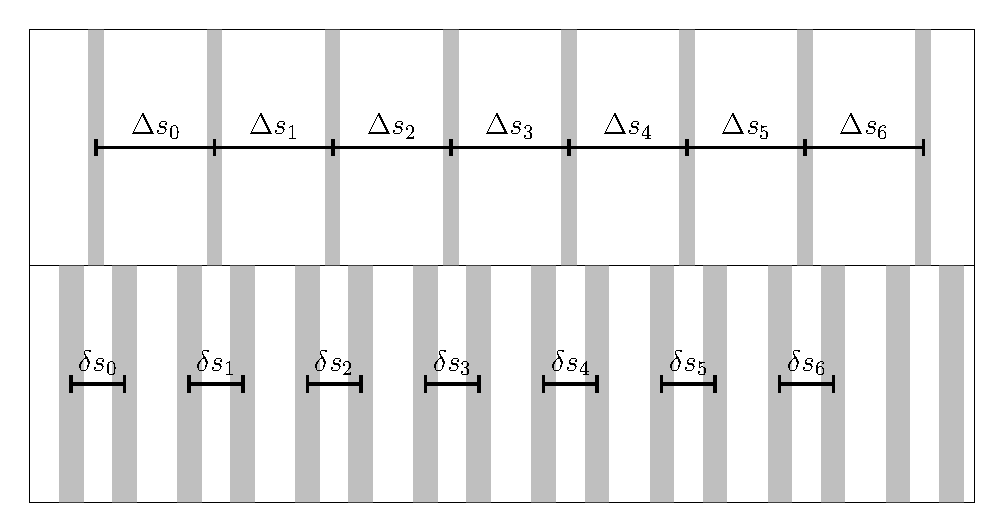
\includegraphics[scale=0.8]{../Grafiken/Messmethode.pdf}
\caption{Schematische Darstellung der Abstände, die in den Aufnahmen der Spekrallinien
        gemessen und für die Auswertung verwendet wurden.\label{fig:messmethode}}
\end{figure}
\FloatBarrier

\FloatBarrier
\begin{figure}[!h]
\centering

\includegraphics[scale=0.1]{../Grafiken/1-I0_t15_sigma_2-I10_t15_sigma.jpg}
\caption{Aufnahmen der roten $\sigma$-Spekrallinie. Im oberen Teil ist die
        Spektrallinie ohne Einfluss eines äußeren Magnetfeldes abgebildet.
        Im unteren Teil ist die Zeemann-Aufspaltung der Spektrallinie
        im äußeren Magnetfeld zu erkennen.\label{fig:1-i0_t15_sigma_2-i10_t15_sigma}}
\end{figure}
\FloatBarrier

\begin{table}[!h]
	\centering
	\begin{tabular}{cccc}
		\toprule
		Linienabstand & Linienabstand & Verhältnis & Wellelängenänderung\\
		$\Delta s$/\si{px} & $\delta s$/\si{px} & $\frac{\delta s}{\Delta s}$ & $\delta \lambda$/\si{\pico\meter}\\
\midrule
		\num{399(5)} & \num{195(5)} & \num{0.49(1)} & \num{11.9(3)}\\
		\num{360(5)} & \num{186(5)} & \num{0.52(2)} & \num{12.6(4)}\\
		\num{337(5)} & \num{168(5)} & \num{0.50(2)} & \num{12.2(4)}\\
		\num{321(5)} & \num{165(5)} & \num{0.51(2)} & \num{12.6(4)}\\
		\num{299(5)} & \num{150(5)} & \num{0.50(2)} & \num{12.3(5)}\\
		\num{289(5)} & \num{144(5)} & \num{0.50(2)} & \num{12.2(5)}\\
		\num{275(5)} & \num{144(5)} & \num{0.52(2)} & \num{12.8(5)}\\
		\num{264(5)} & \num{138(5)} & \num{0.52(2)} & \num{12.8(5)}\\
		\num{253(5)} & \num{128(5)} & \num{0.51(2)} & \num{12.4(5)}\\
		\num{245(5)} & \num{123(5)} & \num{0.50(2)} & \num{12.3(6)}\\
		\num{240(5)} & \num{120(5)} & \num{0.50(2)} & \num{12.2(6)}\\
		\num{231(5)} & \num{114(5)} & \num{0.49(2)} & \num{12.1(6)}\\
		\num{225(5)} & \num{111(5)} & \num{0.49(2)} & \num{12.1(6)}\\
		\bottomrule
	\end{tabular}
	\caption{In Pixeln ausgemessene Abstände $\Delta s$ der unaufgespaltenen  
                                und Abstände $\delta s$ der aufgespaltenen roten Spektrallinien. Zusätzlich sind das
                                Verhältnis dieser Größen und die aus diesem berechnete 
                                Wellenlängenveränderung angegeben. Letztere wurde über \ref{eq:} bestimmt. \label{tab:linienverschiebung}}
\end{table}

\FloatBarrier
\begin{figure}[!h]
\centering

\includegraphics[scale=0.1]{../Grafiken/3-I0_t8_sigma_4-I5_t8_sigma.jpg}
\caption{\label{fig:3-i0_t8_sigma_4-i5_t8_sigma}}
\end{figure}
\FloatBarrier

\begin{table}[!h]
	\centering
	\begin{tabular}{cccc}
		\toprule
		Linienabstand & Linienabstand & Verhältnis & Wellelängenänderung\\
		$\Delta s$/\si{px} & $\delta s$/\si{px} & $\frac{\delta s}{\Delta s}$ & $\delta \lambda$/\si{\pico\meter}\\
\midrule
		\num{392(5)} & \num{213(5)} & \num{0.54(1)} & \num{7.3(2)}\\
		\num{340(5)} & \num{186(5)} & \num{0.55(2)} & \num{7.4(2)}\\
		\num{324(5)} & \num{168(5)} & \num{0.52(2)} & \num{7.0(2)}\\
		\num{292(5)} & \num{153(5)} & \num{0.52(2)} & \num{7.1(3)}\\
		\num{280(5)} & \num{138(5)} & \num{0.49(2)} & \num{6.7(3)}\\
		\num{260(5)} & \num{126(5)} & \num{0.48(2)} & \num{6.5(3)}\\
		\num{248(5)} & \num{119(5)} & \num{0.48(2)} & \num{6.5(3)}\\
		\num{236(5)} & \num{123(5)} & \num{0.52(2)} & \num{7.0(3)}\\
		\num{228(5)} & \num{108(5)} & \num{0.47(2)} & \num{6.4(3)}\\
		\num{220(5)} & \num{111(5)} & \num{0.50(3)} & \num{6.8(3)}\\
		\num{212(5)} & \num{102(5)} & \num{0.48(3)} & \num{6.5(4)}\\
		\num{192(5)} & \num{100(5)} & \num{0.52(3)} & \num{7.0(4)}\\
		\num{198(5)} & \num{93(5)} & \num{0.47(3)} & \num{6.3(4)}\\
		\bottomrule
	\end{tabular}
	\caption{In Pixeln ausgemessene Abstände $\Delta s$ der unaufgespaltenen  
                                und Abstände $\delta s$ der aufgespaltenen blauen $\sigma$-Spektrallinien.
                                Zusätzlich sind das Verhältnis dieser Größen und die aus diesem berechnete 
                                Wellenlängenveränderung angegeben. Letztere wurde über \ref{eq:} bestimmt. \label{tab:linienverschiebung}}
\end{table}

\FloatBarrier
\begin{figure}[!h]
\centering
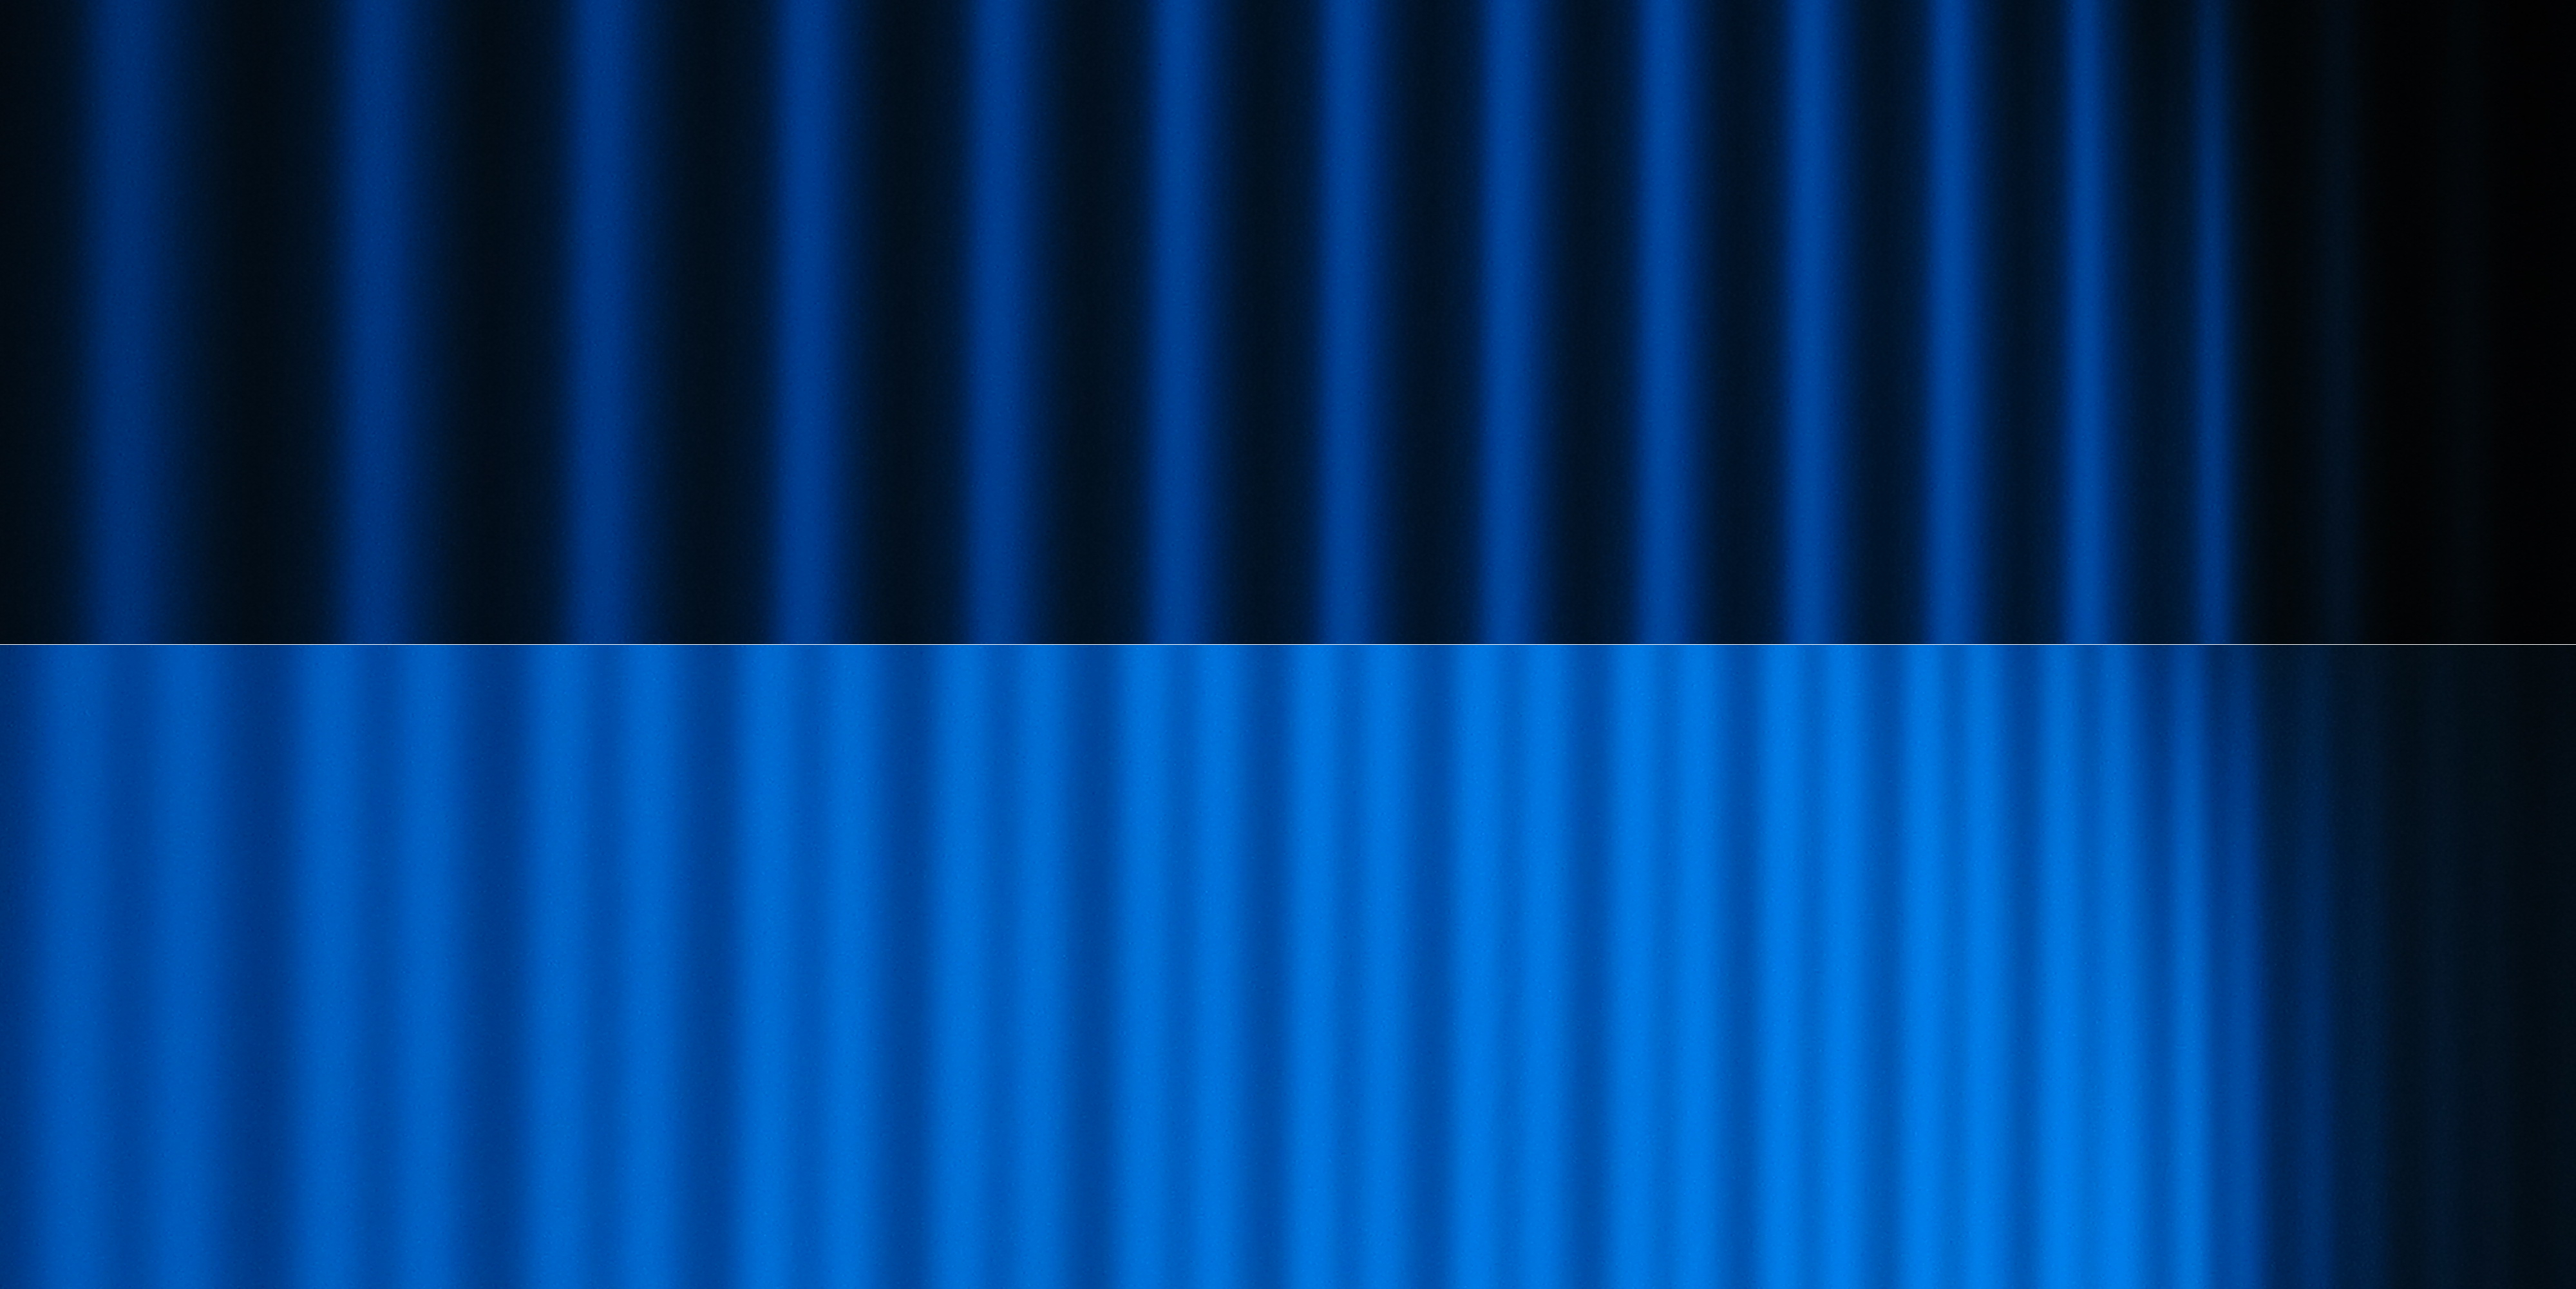
\includegraphics[scale=1]{../Grafiken/5-I0_t8_pi_6-I17_t8_pi.jpg}
\caption{\label{fig:5-i0_t8_pi_6-i17_t8_pi}}
\end{figure}
\FloatBarrier
\begin{table}[!h]
	\centering
	\begin{tabular}{cccc}
		\toprule
		Linienabstand & Linienabstand & Verhältnis & Wellelängenänderung\\
		$\Delta s$/\si{px} & $\delta s$/\si{px} & $\frac{\delta s}{\Delta s}$ & $\delta \lambda$/\si{\pico\meter}\\
\midrule
		\num{387(5)} & \num{192(5)} & \num{0.50(1)} & \num{6.7(2)}\\
		\num{351(5)} & \num{150(5)} & \num{0.43(2)} & \num{5.8(2)}\\
		\num{315(5)} & \num{135(5)} & \num{0.43(2)} & \num{5.8(2)}\\
		\num{297(5)} & \num{123(5)} & \num{0.41(2)} & \num{5.6(2)}\\
		\num{285(5)} & \num{120(5)} & \num{0.42(2)} & \num{5.7(3)}\\
		\num{258(5)} & \num{114(5)} & \num{0.44(2)} & \num{6.0(3)}\\
		\num{252(5)} & \num{114(5)} & \num{0.45(2)} & \num{6.1(3)}\\
		\num{246(5)} & \num{102(5)} & \num{0.41(2)} & \num{5.6(3)}\\
		\num{225(5)} & \num{96(5)} & \num{0.43(2)} & \num{5.8(3)}\\
		\num{219(5)} & \num{87(5)} & \num{0.40(2)} & \num{5.4(3)}\\
		\num{210(5)} & \num{90(5)} & \num{0.43(3)} & \num{5.8(3)}\\
		\num{195(5)} & \num{84(5)} & \num{0.43(3)} & \num{5.8(4)}\\
		\bottomrule
	\end{tabular}
	\caption{In Pixeln ausgemessene Abstände $\Delta s$ der unaufgespaltenen
                                und Abstände $\delta s$ der aufgespaltenen blauen $\pi$-Spektrallinien.
                                Zusätzlich sind das Verhältnis dieser Größen und die aus diesem berechnete
                                Wellenlängenveränderung angegeben. Letztere wurde über \cref{eq:wellenlaengenaenderung} bestimmt.
																\label{tab:linienverschiebung_blau_pi}}
\end{table}


Aus den berechneten Wellenlängenänderungen $\delta \lambda$
wird für jede der drei Spekrallinien eine mittlere Wellenlängenänderung $\mean{\delta \lambda}$
berechnet. Diese ergeben sich zu:

\begin{empheq}{gather*}
  \mean{\delta \lambda}_{\mathrm{rot}-\sigma} = \SI{12.3(1)}{\pico\meter} \\
  \mean{\delta \lambda}_{\mathrm{blau}-\sigma} = \SI{6.81(8)}{\pico\meter} \\
  \mean{\delta \lambda}_{\mathrm{blau}-\pi} = \SI{5.83(8)}{\pico\meter}
\end{empheq}

%(1.23+/-0.01)e-11 m
%(6.81+/-0.08)e-12 m
%(5.83+/-0.08)e-12 m

Aus diesen mittleren Wellenlängenänderungen $\mean{\delta \lambda}$ kann nun
eine Energieänderung $\Delta E$ bestimmt werden. Die Energie ist dabei eine Funktion
der Wellenlänge der Form $E(\lambda) = \mathrm{hc}\lambda^{-1}$.
Die Energieänderung $\Delta E$ ergibt sich nach

\begin{empheq}{align}
  \notag
  \Delta E &= |E(\lambda_{0} + \mean{\delta \lambda}) - E(\lambda_{0})|\\
  \notag
  &= \left|E(\lambda_{0}) + \frac{\partial E}{\partial \lambda}\mean{\delta \lambda} - E(\lambda_{0})\right|\\
  \notag
  &= \left|\frac{\partial E}{\partial \lambda}\mean{\delta \lambda}\right|\\
  \label{eq:energieaenderung}
  &= \frac{\mathrm{hc}}{\lambda^{2}}\mean{\delta \lambda}
\end{empheq}
mit den ensprechenden Wellenlängen $\lambda$ der Spekrallinien aus \cref{tab:Lummer-Gehrcke}.
Nach \cref{eq:anormaler_zeemann_energie} ergibt sich der Lande-Faktor des
Übergangs $g_{ij}$ aus der Energieänderung $\Delta E$ durch die Umformung

\begin{empheq}{align}
  \notag
  \Delta E &= g_{ij} \cdot \mu_{\mathrm{B}}\cdot B\\
  \label{eq:lande_energieaenderung}
  \Leftrightarrow g_{ij} &= \frac{\Delta E}{\mu_{\mathrm{B}}\cdot B}.
\end{empheq}


\begin{table}[!h]
	\centering
	\begin{tabular}{lcccc}
		\toprule
		Messung & Energieänderung & Lande-Faktor & Lande-Faktor (theo.) & rel. Abweichung\\
		 & $\Delta E$/\si{10\tothe{-24}\joule} & $g_{ij}$ & $g_{ij,\mathrm{theo}}$ & $\frac{|g_{ij} - g_{ij,\mathrm{theo}}|}{g_{ij,\mathrm{theo}}}$/\si{\percent}\\
\midrule
		rot $\sigma$ & \num{5.91(7)} & \num{1.08(5)} & \num{1} & \num{7(5)}\\
		blau $\sigma$ & \num{5.87(7)} & \num{2.0(2)} & \num{2} & \num{2(10)}\\
		blau $\pi$ & \num{5.02(7)} & \num{0.55(2)} & \num{0.5} & \num{10(4)}\\
		\bottomrule
	\end{tabular}
	\caption{Unter Verwendung von \cref{eq:energieaenderung} aus der mittleren Wellenlängenveränderung $\mean{\delta \lambda}$
                          berechnete Energieänderung $\Delta E$ und die entsprechenden Lande-Faktoren nach \cref{eq:lande_energieaenderung}.
                          Zusätzlich sind die theoretischen Lande-Faktoren und die relativen Abweichungen
                          der berechneten Lande-Faktoren angegeben. \label{tab:lande_ergebnis}}
\end{table}

